\documentclass{scrartcl}

% packages
\usepackage{amsmath}
\usepackage{amssymb}
\usepackage[ngerman]{babel}
\usepackage{booktabs}
\usepackage[font=small,labelfont=bf]{caption}
\usepackage{csquotes}
\usepackage{float}
\usepackage{fontspec}
  \setmainfont[Ligatures=TeX]{Tex Gyre Pagella}
\usepackage{graphicx}
\usepackage[pdfusetitle,unicode]{hyperref}
\usepackage{mathtools}
\usepackage{microtype}
\usepackage{siunitx}
  \sisetup{separate-uncertainty=true}
\usepackage{subcaption}
\usepackage[math-style=ISO,bold-style=ISO]{unicode-math}
  \setmathfont{Tex Gyre Pagella Math}
\usepackage{xfrac}

% options
\setlength{\parindent}{0pt}  % no stupid indentation

% commands
\DeclarePairedDelimiter{\abs}{\lvert}{\rvert}
\DeclarePairedDelimiter{\mean}{\langle}{\rangle}
\renewcommand{\vec}[1]{\mathbf{#1}}
\renewcommand{\i}{\mathrm{i}}
\DeclareRobustCommand{\e}{\ensuremath{\mathrm{e}}}

% meta
\author{Kevin Dungs \and Kevin Heinicke \and Holger Stevens}
\title{Computational Physics}
\subtitle{Übungsblatt 4}

% document
\begin{document}
\maketitle

\section*{Hausaufgabe 9: Sampling und Integration in hohen Dimensionen}
\paragraph{(a)} Das Volumen der $d$-dimensionalen Einheitskugel ist
\begin{equation}
    V_S(d) = \frac{\pi^{\sfrac{d}{2}}}{\Gamma(1 + \sfrac{d}{2})}
\end{equation}
In \autoref{fig:analytical} ist der Verlauf des Zusammenhangs für $d=1\dots200$ dargestellt.

\begin{figure}[H]
    \centering
    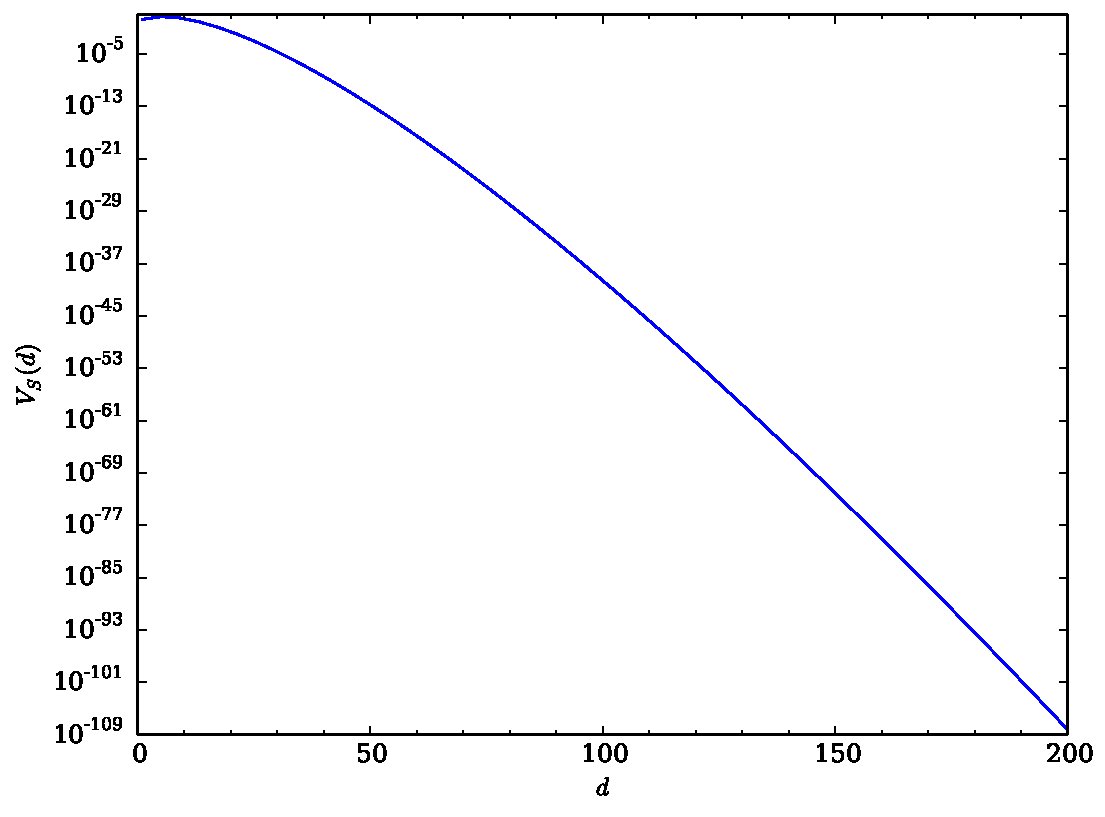
\includegraphics[width=0.5\textwidth]{plots/analytical.pdf}
    \caption{Volumen der Einheitskugel in Abhängigkeit der Dimension.}
    \label{fig:analytical}
\end{figure}

\paragraph{(b)} Für $d=200$ müssen \num{200} Zufallszahlen gezogen und deren Quadratsumme berechnet werden. Das allein ist schon ein aufwändiger Prozess. Dazu kommt, dass das Verhältnis der Volumina von $d$-dimensionalem Hyperwürfel und $d$-dimensionaler Kugel immer drastischer auseinander geht und somit mit steigender Dimension immer mehr Würfe verworfen werden.

\paragraph{(c)}
\paragraph{(d)}

\end{document}
